%% 
%% Copyright 2019 Elsevier Ltd
%% 
%%
%%%%%%%%%%%%%%%%%%%%%%%%%%%% ! ! ! SUBMISSION CHECKLIST ! ! ! %%%%%%%%%%%%%%%%%%%%%%%%%%%%
%%
%% Please confirm that your submission follows all the requirements of the guidelines, including the submission checklist:
%% _ Cover letter
%% _ Highlights
%% _ Authorship statement
%% _ The manuscript must be single column and double spaced
%% _ Reference must be in the author-date format
%% _ Code availability section 
%%
%% *All the manuscripts in disagreement with the guidelines will be desk-rejected without editorial check.
%%
%% --------------------------------------
%%
%% This file is part of the 'CAS Bundle'.
%%  
%% It may be distributed under the conditions of the LaTeX Project Public
%% License, either version 1.2 of this license or (at your option) any
%% later version.  The latest version of this license is in 
%%    http://www.latex-project.org/lppl.txt 
%% and version 1.2 or later is part of all distributions of LaTeX
%% version 1999/12/01 or later.
%%   
%% The list of all files belonging to the 'CAS Bundle' is
%% given in the file `manifest.txt'.
%% 
%% Template article for cas-dc documentclass for  
%% double column output.
 
%\documentclass[a4paper,fleqn,longmktitle]{cas-dc}
\documentclass[a4paper,fleqn]{cas-sc}

\usepackage[authoryear]{natbib}
\usepackage{graphicx} 
\usepackage{float}
\usepackage{algorithm}  
\usepackage{algpseudocode}
\usepackage{color}
\usepackage{setspace}
\usepackage[nomarkers,figuresonly]{endfloat}


\newcommand{\colorComments}{black} 
 
%%%Author definitions
\def\tsc#1{\csdef{#1}{\textsc{\lowercase{#1}}\xspace}}
\tsc{WGM}
\tsc{QE}
\tsc{EP}
\tsc{PMS}
\tsc{BEC}
\tsc{DE}
%%%

\usepackage{lineno}
\linenumbers 

\begin{document}
\let\WriteBookmarks\relax
\def\floatpagepagefraction{1}
\def\textpagefraction{.001}
\shorttitle{Short title}
\shortauthors{short author name}

\title [mode = title]{Flooding based mobilenet v3 identifies cucumber isease leaves in fuzzy scenes  }


\author[1]{Author 1}[type=editor,
                        auid=000,bioid=1,orcid=0000-0000-0000-0000]
\credit{ Author 1 contribution  }

\author[2]{Author 2} 
\credit{Author 2 contribution }

\author[3]{Author 3}
\credit{Author 3 contribution}

\address[1]{Author 1 affiliation}
\address[2]{Author 2 affiliation}
\address[3]{Author 3 affiliation} 

\begin{abstract}
Abstract text here, abstract text here,  abstract text here,  abstract text here,  abstract text here,  abstract text here,  abstract text here,  abstract text here,  abstract text here,  abstract text here,  abstract text here,  abstract text here,  abstract text here,  abstract text here,  abstract text here,  abstract text here,  abstract text here,  abstract text here,  abstract text here.
\end{abstract}
 
% \begin{coverletter}

% Dear Editors-in-Chief,
% \newline
 
% please find the enclosed manuscript "..." which we are submitting for exclusive consideration for publication in Computers \& Geosciences. We confirm that the submission follows all the requirements and includes all the items of the submission checklist.  
% \newline
 
% The manuscript presents ... 
% \newline

% We provide the source codes in a public repository with details listed in the section "Code availability".
% \newline

% Thanks for your consideration. 
% \newline

% Sincerely,
% \newline

% Authors names

% Corresponding author affiliation and e-mail
% \newline

% \textbf{Delete before submission:}

% Please confirm that your submission follows all the requirements of the guidelines, including the submission checklist:

% - Cover letter

% - Highlights

% - Authorship statement

% - The manuscript must be single column and double spaced

% - Reference must be in the author-date format

% - Code availability section 

% *The manuscripts that do meet the requirement guidelines will be desk-rejected.



% \end{coverletter}

 
% \begin{highlights}
% \item Highlight 1
% \item Highlight 2
% \item Highlight 3
% \item Highlight 4
% \item Highlight 5
% \end{highlights}

\begin{keywords}
Keyword 1 \sep Keyword 2 \sep Keyword 3 \sep Keyword 4
\end{keywords}

\maketitle 

\printcredits

\doublespacing


\section{Introduction}
\label{intro}



Examples of citations:

\cite{gomez1990isim3d, pebesma2004multivariable, hansen2018multiple}

Examples of citations in parentheses: 

\citep{gomez1990isim3d, pebesma2004multivariable, hansen2018multiple}

\section{Methodology}

This section includes an example of equation. 
 
\begin{equation}
\label{eqn:linear}
    y=ax+b.
\end{equation}


\subsection{Subsection}

This section contains another example of equation, different from Eq.  \ref{eqn:linear}.

\begin{equation} 
\label{eqn:quadratic}
    y=ax^2+bx+c
\end{equation}

\section{Algorithm and implementation}

Example of algorithm:
\begin{algorithm}
  \caption{Algorithm example }
  
  \begin{algorithmic}
  \label{alg:Alg1}
  \State \textbf{Input:} ...
   \newline

 \Statex \textit{1.} Step1
  \Statex \textit{2.} Step2;
 \State \textit{3.}  Step3;
  \newline
   \For{ i = 1,..., m}
   \State \textit{4.} Step 4;
    \For{ j = 2,..., n} 
   \State \textit{5.}  Step 5;
   \State \textit{6.} Step 6;
   \EndFor
  \EndFor 
  \newline
\State  \textbf{Output: } ... 
  \end{algorithmic} 
\end{algorithm} 


\section{Results}


This section includes an example of figure (Figure \ref{fig:Figure1}), from  \cite{de2021direct}.

\begin{figure}
\centering
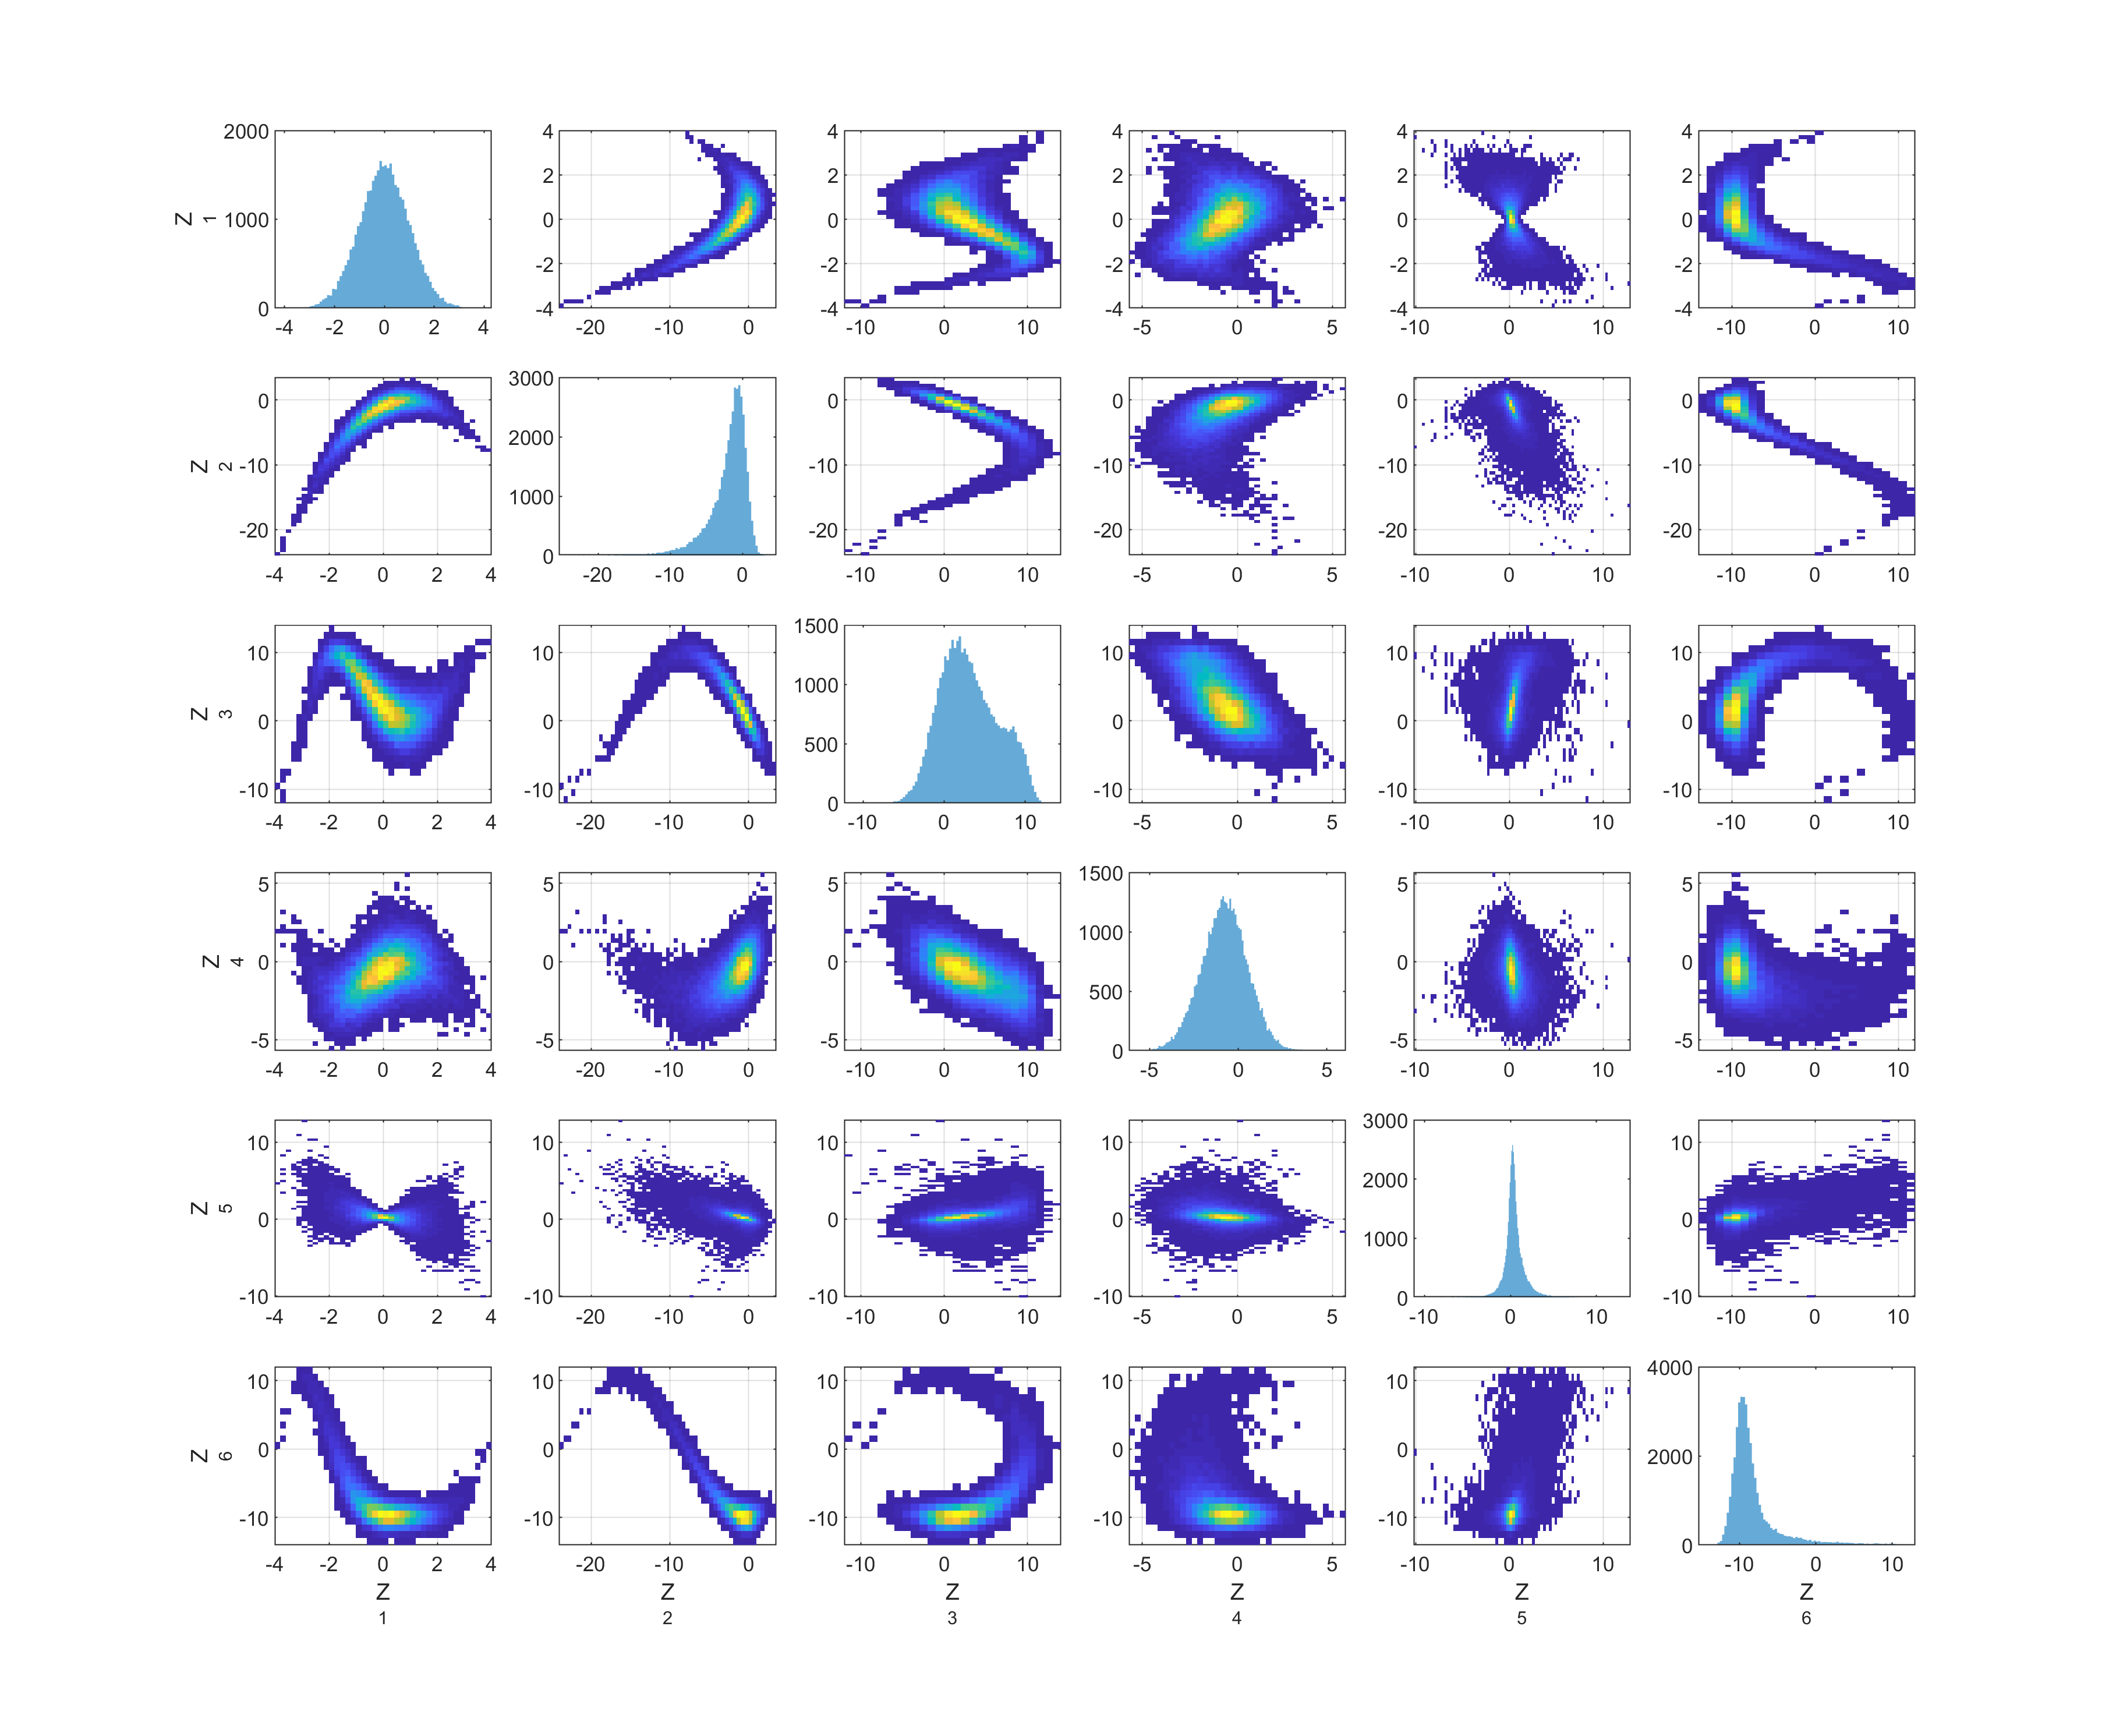
\includegraphics[width=0.75\textwidth]{figs_rev1/uncond_distribution_reference.png}
\caption{ Caption here. Image from \cite{de2021direct}.}
\label{fig:Figure1}
\end{figure}

This section includes an example of table (Table \ref{tab:Table1}).

\begin{table}
\centering
\caption{Example of table.}
\label{tab:Table1}
\begin{tabular}{ |c||c|c|c|} 
 \hline
     & $a$  &  $b$  &  $c$\\ 
 \hline 
 \hline
$a$ & 0.014 &  0.20    &   0.13  \\
\hline
$b$ & 0.20    &   0.17    &   2.46    \\
\hline
$c$ & 0.13    &   2.5     &   0.31   \\
\hline
\end{tabular} 
\end{table}


\subsection{Subsection}

Text ...

\section{Conclusions}

Conclusions here...

\section{Acknowledgments}

The authors would like to acknowledge ...

\newpage

\textbf{Code availability section}

Name of the code/library

Contact: e-mail and phone number

Hardware requirements: ...

Program language: ...
 
Software required: ...

Program size: ...

The source codes are available for downloading at the link:
https://github.com/ . . . . 


\bibliographystyle{cas-model2-names}
\bibliography{bibliography} 

\end{document}

